\documentclass[10pt, a4paper]{beamer}
\usepackage{ragged2e}
\usepackage{tabularray}
\usepackage[none]{hyphenat}

\usetheme{Berkeley}
\usecolortheme{sidebartab}
\graphicspath{{./images/}}

\begin{document}
	\setbeamertemplate{sidebar left}{}
	\title{Project Presentation}
	\subtitle{e-Yantra Summer Internship-2022 \\ 53 - FPGA for Edge}
	\author{Anupam Kurien Mathew\\Dan Mani Binu\\Hari Vikinesh\\\vspace{0.3cm}\textbf{Mentors:} Isha Kamone, Lohit Penubaku}
	\institute{IIT Bombay}
	\date{July 25, 2022}
	\frame{\titlepage}

\setbeamertemplate{sidebar left}[sidebar theme]
\section{Overview of Project}
\begin{frame}{Overview of Project}
	\begin{itemize}
		\item Objective \\
				\justifying\hspace{7.5mm}The aim of the project is to understand and exploit the potential of FPGAs in the application of agriculture. The work will focus on training ML models which can be deployed on FPGA, and video processing to use the ML models for indoor agricultural applications.
		\item Hardware - Zedboard \& Nexys Video Development Kit and OV7670 Camera
		\item Software - Xilinx Vivado, Vivado HLS, Paperspace
		\item Deliverables \\
			\begin{enumerate}
				\item Model for tomato leaf detection
				\item Comparison of performance of model on CPU, GPU \& FPGA
				\item Proper Documentation and Report
			\end{enumerate}
	\end{itemize}
\end{frame}

\section{Overview of Task}
\begin{frame}{Overview of Task}
	\begin{table}[!h]
		\resizebox{\textwidth}{!}{%
		\small
		\begin{tblr}{|Q[c, 15mm]|Q[j, 80mm]|Q[c, 20mm]|}
			\hline
			\textbf{Task No.} & \centering \textbf{Tasks} & \textbf{Time Provided} \\ \hline
			1 & Read existing research Papers & 3 Days \\ \hline
			2 & Familiarizing with the work done in earlier eYSIP project & 1 Week \\ \hline
			3 & Detection of Tomato leaves algorithm using existing datasets \& making note of performance with and without GPU & 1 Week \\ \hline
			4 & Exploring FPGA boards \& interfacing Camera & 1 Week \\ \hline
			5 & Implementation of Lane Detection Algorithm & 1 Week \\ \hline
			6 & Testing Edge Detection techniques in the previous tasks on tomato leaves & 3 Days \\ \hline
			7 & Running tomato leaf algorithm on FPGA \& measuring the same performance parameters & 4 Days \\ \hline
			8 & Tuning the algorithm to better the performance seen with GPU & 3 Days \\ \hline
			9 & Documentation, Code Commenting, Report & 1 Week \\
			\hline
		\end{tblr}}
		\caption{Timeline of the project}
	\end{table}
\end{frame}

\section{Literature Review}
% \begin{frame}{Task Accomplished}
% 	\begin{itemize}
% 		\item \href{https://docs.google.com/spreadsheets/d/1vpyTfLYproK1xdVhq1EVYxqp-3dGCHk7qDcSNgZSEWk/edit?usp=sharing}{\underline{Studied}} various Research Papers focusing on \\
% 			\begin{enumerate}
% 				\item Developing ML accelerators.
% 				\item Comparing performance of FPGA with CPU \& GPU.
% 			\end{enumerate}
% 		\item Understood Previous year eYSIP projects.
% 		\item Learnt to use Xilinx Vivado and Vitis HLS.
% 		\item Developed a basic tomato leaf detection model (Yolo-v3-tiny, Yolo-v5, mask-r-CNN).
% 		\item Implemented basic circuits using verilog and HLS with Zedboard/Nexys Video.
% 	\end{itemize}
% \end{frame}

\begin{frame}{Hardware Accelerators on FPGA}
	\begin{table}
		\centering
		\resizebox{\textwidth}{!}{
		\small
		\begin{tblr}{|Q[c,25mm]|Q[c,15mm]|Q[c,15mm]|Q[c,15mm]|Q[c,15mm]|Q[c,15mm]|Q[c,15mm]|Q[c,15mm]|}
			\hline
			\textbf{Platform} & Zynq XC7Z045 & Xilinx Zynq ZC702 & Stratix-V & Zynq Ultrascale+ & Intel Arria 10 GX115 & Virtex-7 VC707 & Kintex Ultrascale XCKU115 \\ \hline
			Frequency (MHz) & 200 & 100 & 150 & 200 & 200 & 200 & 125 \\
			BRAMs (KB) & 186 & 630 & 2210 & 1824 & 2232 & 1214 & 1814 \\
			DSPs & - & 140 & 384 & 2520 & 1518 & 272 & - \\
			LUTs & 46.3K & 36.1k & 230.9K & 600K & 138K & 104.7K & 392.9K \\
			FFs & - & 36.8K & 350K & - & 823.4K & 140.1K & 348K \\
			CNN Size & 0.1125 & 14.5 & 1.45 & 5 layers of VGG & 30.95 & 30.74 & 1.2 \\
			Precision(W, A) & (1, 1) & (1, 1) & (1, 1) & (16, 16) & (16, 16) & (1, 2) & (1, 1) \\
			Image Size & 32x32 & - & 224x224 & 224x224 & 224x224 & 224x224 & 32x32 \\
			Throughput (GOPS) & 2463.8 & - & 1964 & 2940.7 & 715.9 & 4420 & 14814 \\
			Efficiency (GOPS/kLUT) & 53.2 & - & 8.51 & 4.9 & 5.19 & 42.22 & 37.7 \\
			Power (W) & 11.7 & - & 26.2 & 23.6 & - & 14.72 & - \\
			Power efficiency (GOPs/W) & 210.58 & - & 74.96 & 124.6 & - & 300.27 & - \\ \hline
		\end{tblr}}
		\caption{DNN Hardware Accelerators}
	\end{table}
\end{frame}

\begin{frame}{Performance Analysis}
	\begin{figure}
		\centering
		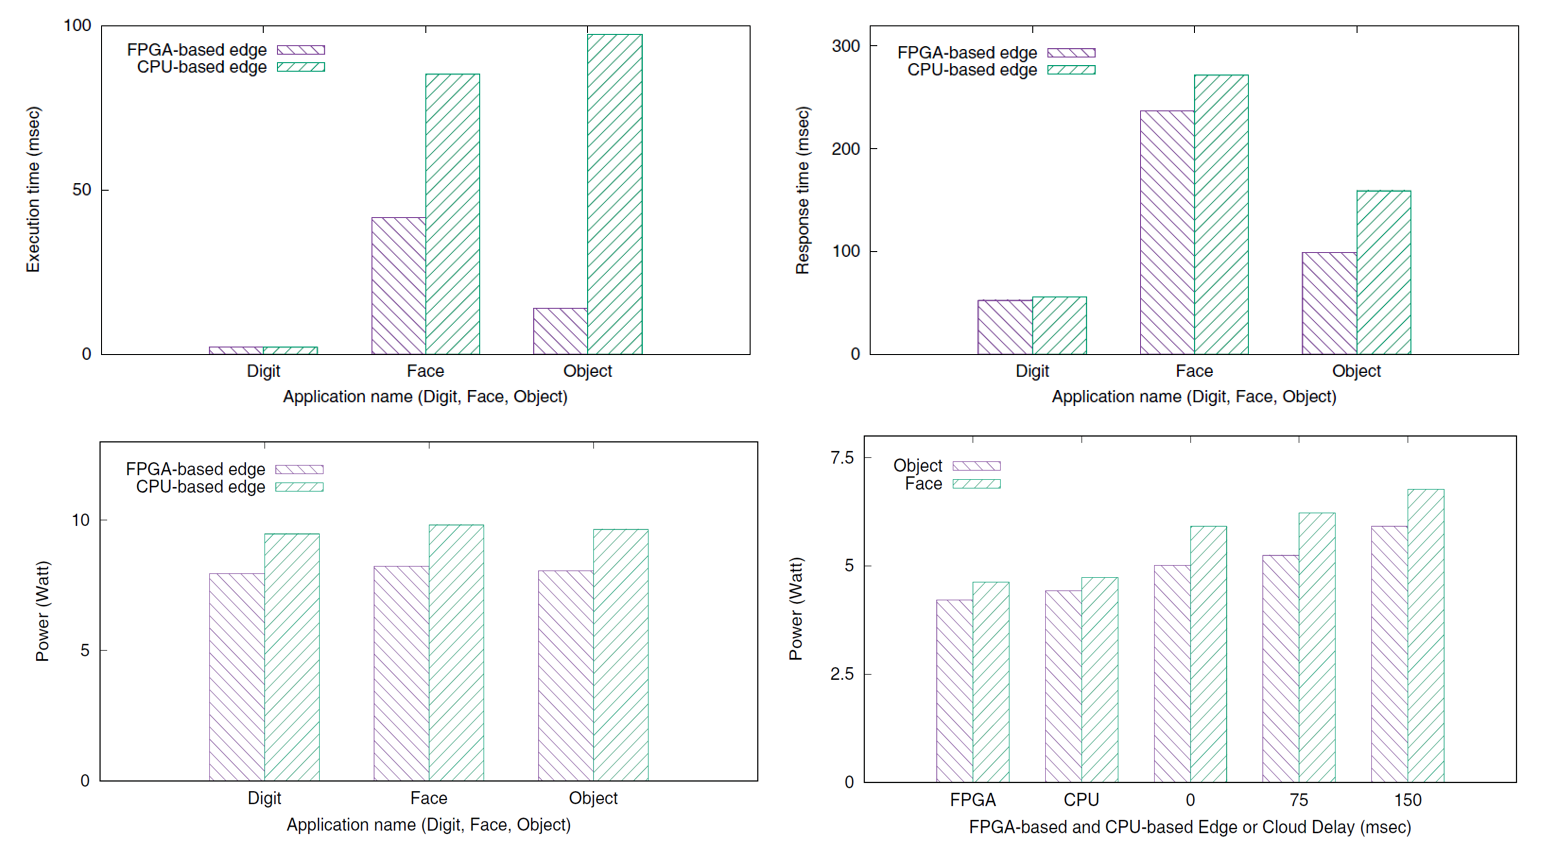
\includegraphics[width=\linewidth]{performance}
		\caption{Performance Comparison between FPGA, CPU \& GPU}
	\end{figure}
\end{frame}

% \subsection{Previous year eYSIP work}
\begin{frame}{Previous year eYSIP work}
	\begin{figure}
		\centering
		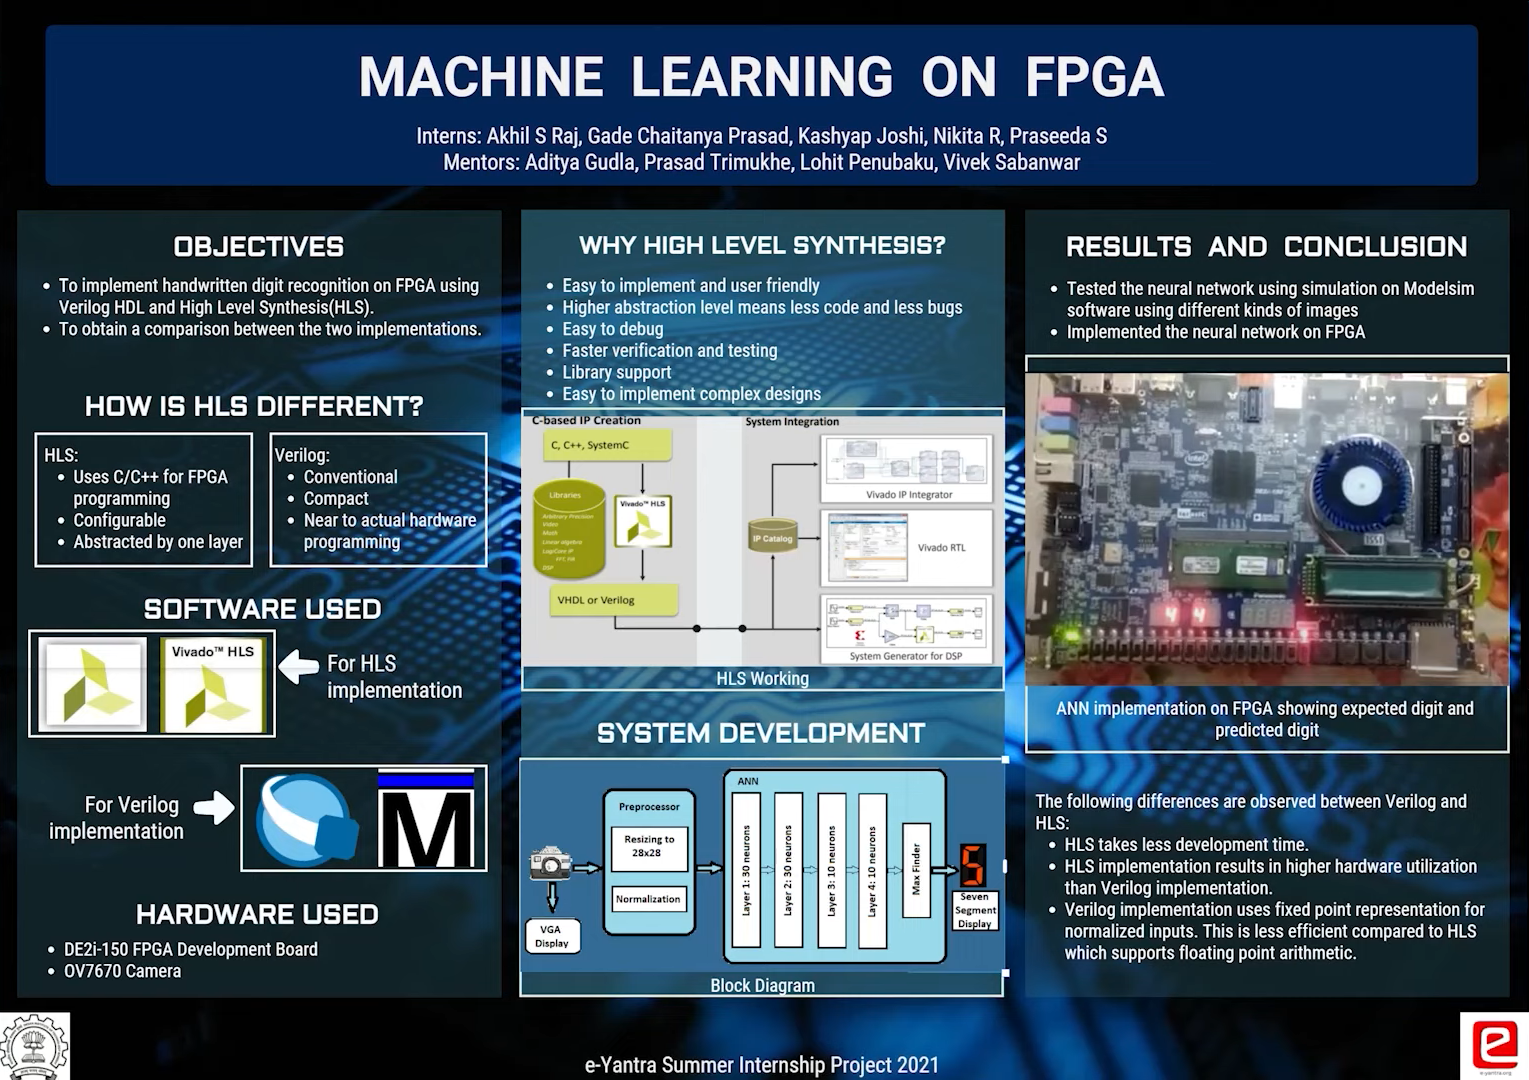
\includegraphics[scale=0.235]{eYSIP-21}
		\caption{ML on FPGA}
	\end{figure}
\end{frame}

\section{Approach}
\subsection{ML Models}
\begin{frame}{Object Detection Models}
	\begin{figure}
		\centering
		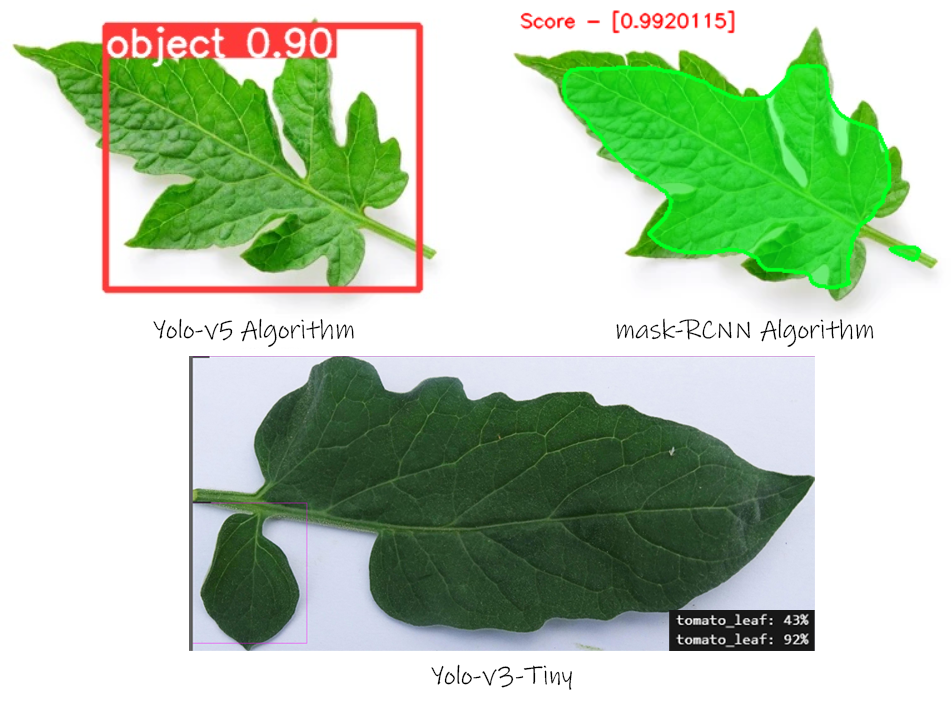
\includegraphics[scale=0.25]{models}
		\caption{Results for various tomato leaf detection models}
	\end{figure}
\end{frame}

\subsection{Xilinx FPGAs}
\begin{frame}{Understanding Xilinx FPGAs}
	\begin{figure}
		\centering
		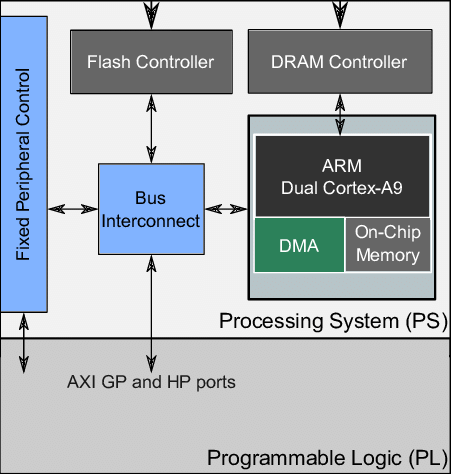
\includegraphics[scale=0.40]{xilinx-fpga}
		\caption{Xilinx Internal Architecture}
	\end{figure}
\end{frame}

\subsection{Edge Detection}
\begin{frame}{Lane Detection}
	Sobel Algorithm
	\begin{itemize}
		\item \justifying The Sobel operator performs a 2-D spatial gradient measurement on an image and so emphasizes regions of high spatial frequency that correspond to edges.
	\end{itemize}
	\begin{figure}
		\centering
		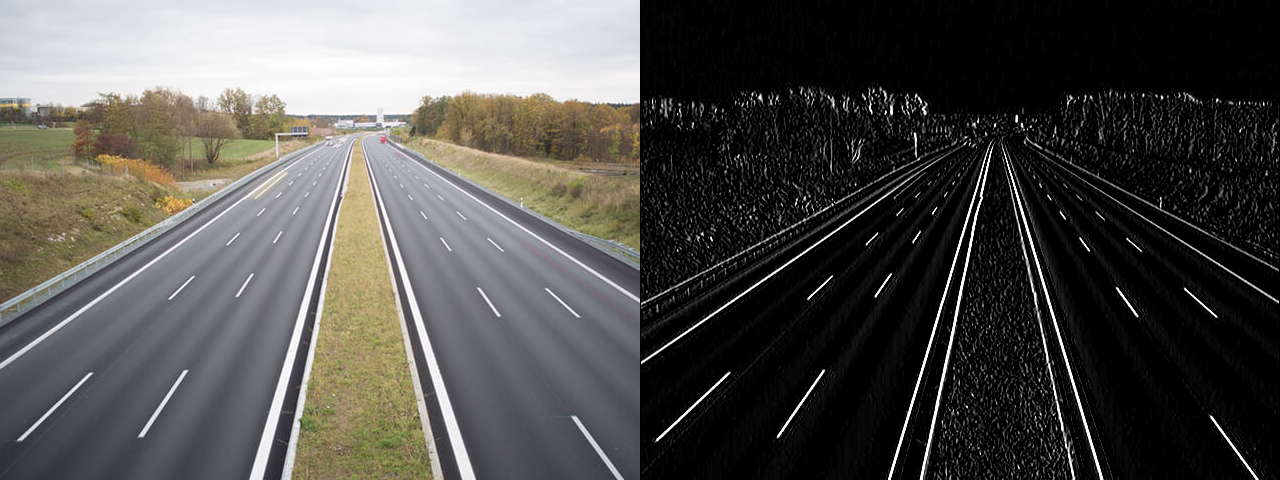
\includegraphics[scale=0.20]{laneresult}
		\caption{Lane Detection Result}
	\end{figure}
\end{frame}

\begin{frame}{Edge Detection on Tomato Leaves}
	\begin{itemize}
		\item Edge Detection \& Feature Extraction
	\end{itemize}
	\begin{figure}
		\centering
		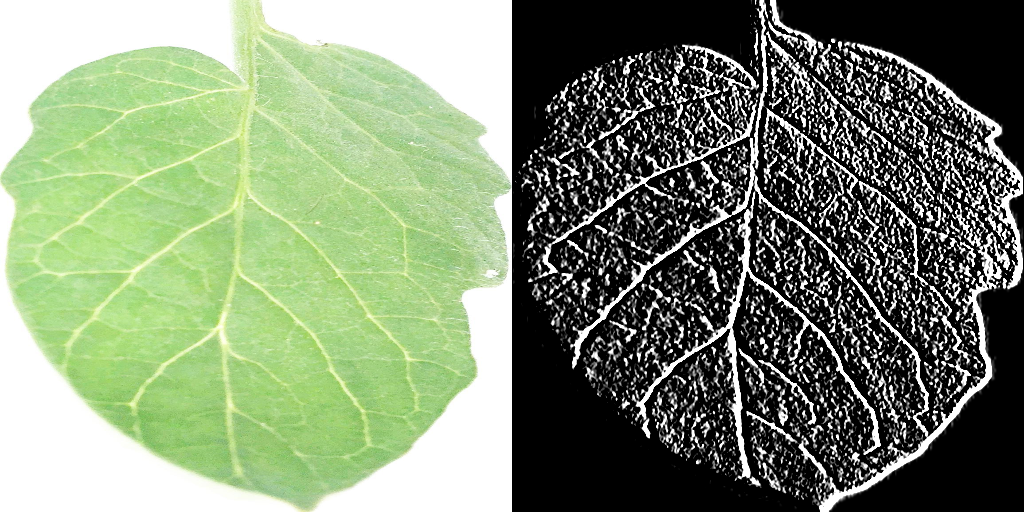
\includegraphics[scale=0.275]{leafresult}
		\caption{Tomato Leaf Edge Detection Result}
	\end{figure}
\end{frame}

\subsection{Accelerator Development}
\begin{frame}{YOLOv2 Model}
	\begin{itemize}
		\item what is YOLO?\\
		\justifying \hspace{7.5mm} You Only Look Once(YOLO) algorithm detects and recognizes various objects in a picture. YOLO algorithm employs convolutional neural networks (CNN) to predict various class probabilities and bounding boxes simultaneously. This algorithm requires only a single forward propagation through a neural network to detect objects. This means that prediction in the entire image is done in a single algorithm run.
		\item why YOLO?\\
		\begin{itemize}
			\item Learning Capabilities
			\item High Accuracy
			\item Speed
		\end{itemize}
	\end{itemize}
\end{frame}

\begin{frame}{YOLOv2-Tiny Architecture}
	\begin{figure}
		\centering
		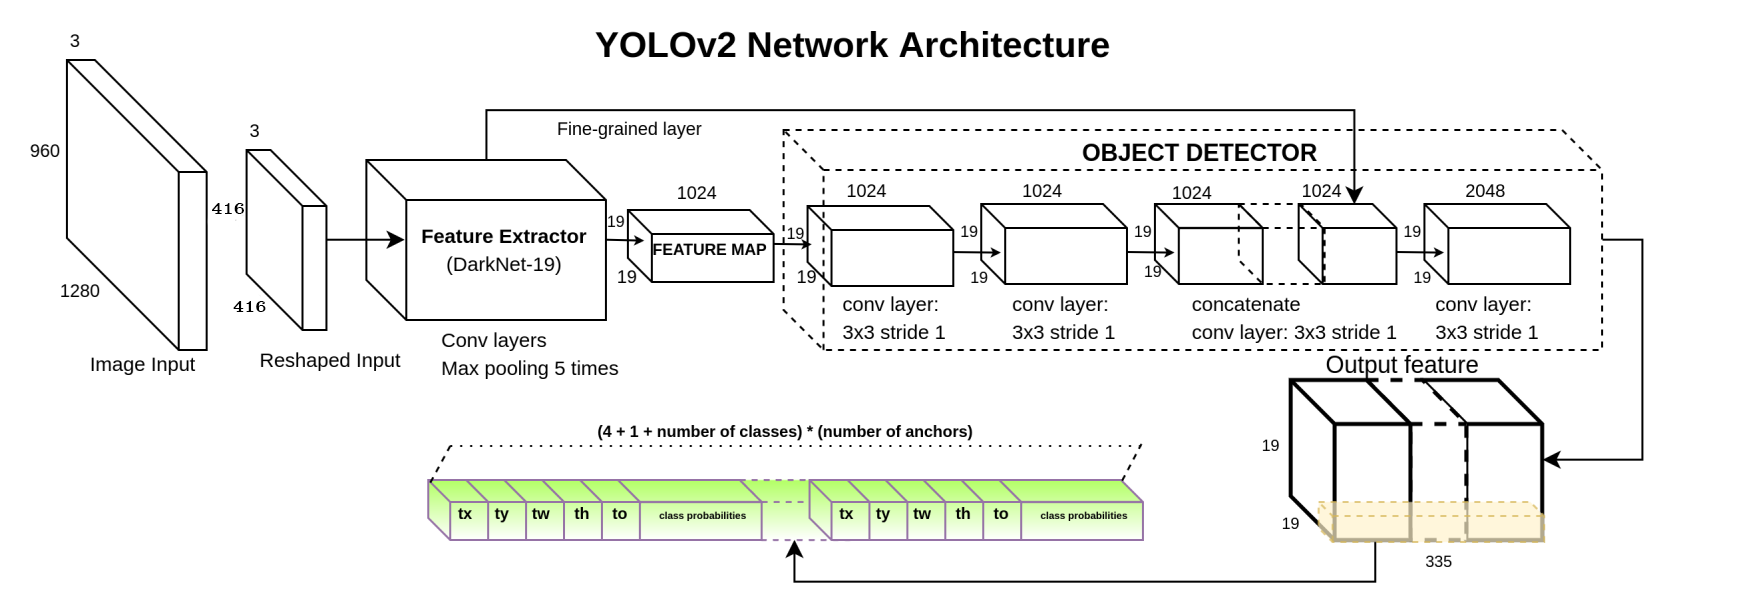
\includegraphics[scale=0.175]{yolov2-architecture}
		\caption{Architecture of Yolov2 Model}
	\end{figure}
\end{frame}

% \begin{frame}{Top Level Design}
% 	\begin{figure}
% 		\centering
% 		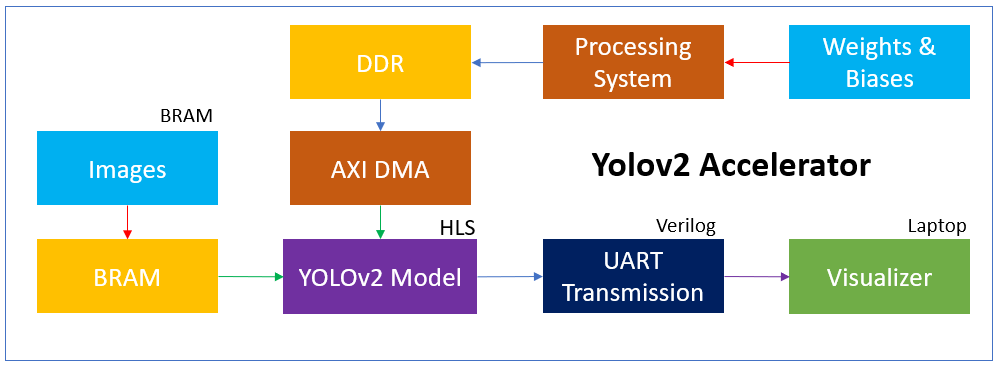
\includegraphics[width=\linewidth]{Accelerator}
% 		\caption{Architecture Representing DataFlow}
% 	\end{figure}
% \end{frame}

\section{Performance Analysis}
\begin{frame}{Performance Comparison with Traditional Hardwares}
	\begin{figure}
		\centering
		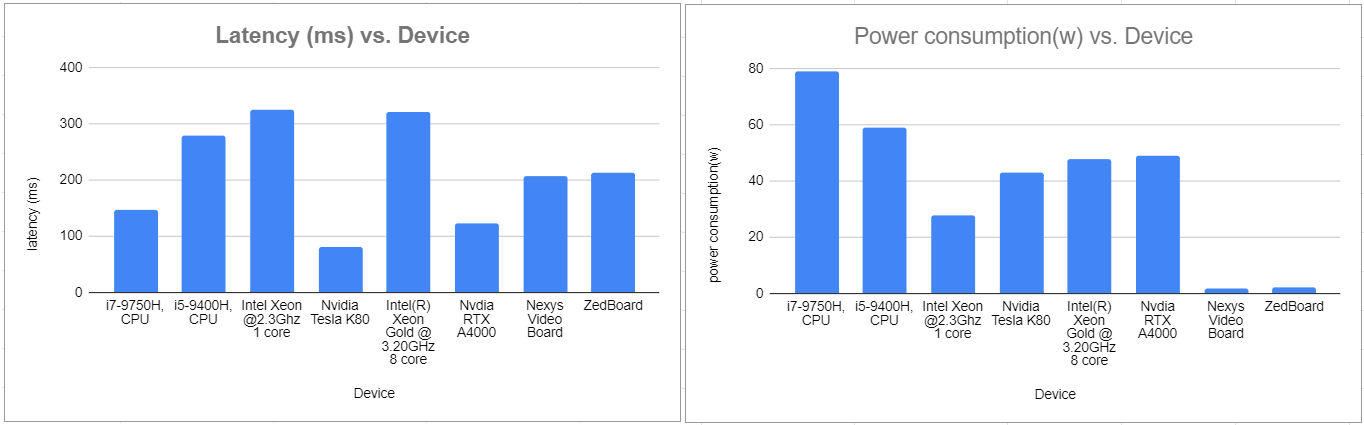
\includegraphics[width=\linewidth]{performance-plus}
		\caption{Comparison between FPGA, CPU \& GPU}
	\end{figure}
\end{frame}

\begin{frame}{Performance Comparison with Existing Accelerators}
	\begin{table}
		\centering
		\caption{Comparison with Hardware Accelerators}
		\resizebox{\textwidth}{!}{
		\small
		\begin{tblr}{|Q[c,25mm]|Q[c,15mm]|Q[c,15mm]|Q[c,15mm]|Q[c,15mm]|Q[c,15mm]|Q[c,15mm]|Q[c,15mm]|Q[c,15mm]|Q[c,15mm]|}
		\hline
		\textbf{Platform}         & Zynq XC7Z045 & Xilinx Zynq ZC702 & Kintex Ultrascale XCKU115 & Stratix-V   & Virtex-7 VC707     & Zynq Ultrascale+ & Intel Arria 10 GX115 & ZedBoard (This work) & Nexys Video (This work) \\ \hline
		Frequency (MHz)           & 200          & 100               & 125                       & 150         & 200                & 200              & 200                  & 100                  & 100                     \\
		BRAMs (KB)                & 186          & 630               & 1814                      & 2210        & 1214               & 1824             & 2232                 & 810                  & 890                     \\
		DSPs                      & -            & 140               & -                         & 384         & 272                & 2520             & 1518                 & 139                  & 148                     \\
		LUTs                      & 46.3K        & 36.1k             & 392.9K                    & 230.9K      & 104.7K             & 600K             & 138K                 & 51.4K                & 40.2K                   \\
		FFs                       & -            & 36.8K             & 348K                      & 350K        & 140.1K             & -                & 823.4K               & 31.4K                & 31.4K                   \\
		CNN Size                  & 0.1125       & 14.5              & 1.2                       & 1.45        & 30.74              & 5 layers of VGG  & 30.95                & 42.3                 & 42.3                    \\
		Precision                 & 8-bit fixed  & 8-bit fixed       & 8-bit fixed               & 8-bit fixed & (8-16)bit fixed    & 16-bit fixed     & 16-bit fixed         & 32-bit float         & 32-bit float            \\
		Image Size                & 32x32        & -                 & 32x32                     & 224x224     & 224x224            & 224x224          & 224x224              & 64x64                & 64x64                   \\ \hline
		\end{tblr}}
	\end{table}
\end{frame}

\section{Conclusion}
\begin{frame}{Conclusion}
	\begin{itemize}
		\item  From the comparisons, it is evident that ML model implementation
	works best on FPGAs and GPUs.
		\item  The choice between FPGA and GPU is application specific and FPGAs are best for low-power implementation and standalone applications.
		\item  A more efficient code can alter the speed and resources required to implement the model.

		\item Traditional hardware like CPUs has turned out to be poor choices for model implementation.
		\item Based on the resource cost and simple architecture the propsed model can be implemented on low-tier FPGAs.
	\end{itemize}
\end{frame}

\section{Thank You}
\begin{frame}{Thank You}
	\begin{figure}
		\centering
		
\includegraphics[scale=1.25]{thankyou}
	\end{figure}
\end{frame}

\end{document}
